\chapter{Standard Model and Top Quark Physics}
\label{Chapter2}
\section{Introduction to Standard Model of Particle Physics}
\label{SM}
The Standard Model of Particle Physics classifies all the known elementary particles and describes the interaction between them. It fully characterizes the three out of four known fundamental forces; electromagnetic, weak, and strong. The gravitational interaction not included in the SM. In the mid-1970s, the current formulation of the SM was completed, and the first observation of the quarks in 1968 was a bold, experimental proof of the SM. Since then, many more experiments have confirmed the predictions of the SM, and the latest was Higgs boson discovery in 2012 confirmed by ATLAS \cite{20121} and CMS \cite{201230} collaborations based on the proton-proton collisions in the LHC at CERN.

The elementary particles divided into different classes depending on their distinguishable properties such as spin, color charge, and flavor. They fall into two major categories of fermions and bosons according to their spin angular momentum. The fermions are spin-half particles, and the bosons have integer spin. The fermions further classify as quarks (\textit{q}) and leptons (\textit{l}) according to how they interact. The vector gauge bosons (spin = 1) and scaler boson (spin = 0) are two classes of bosons. The gauge bosons are known as the force carriers in the SM.

\begin{figure}
\centering
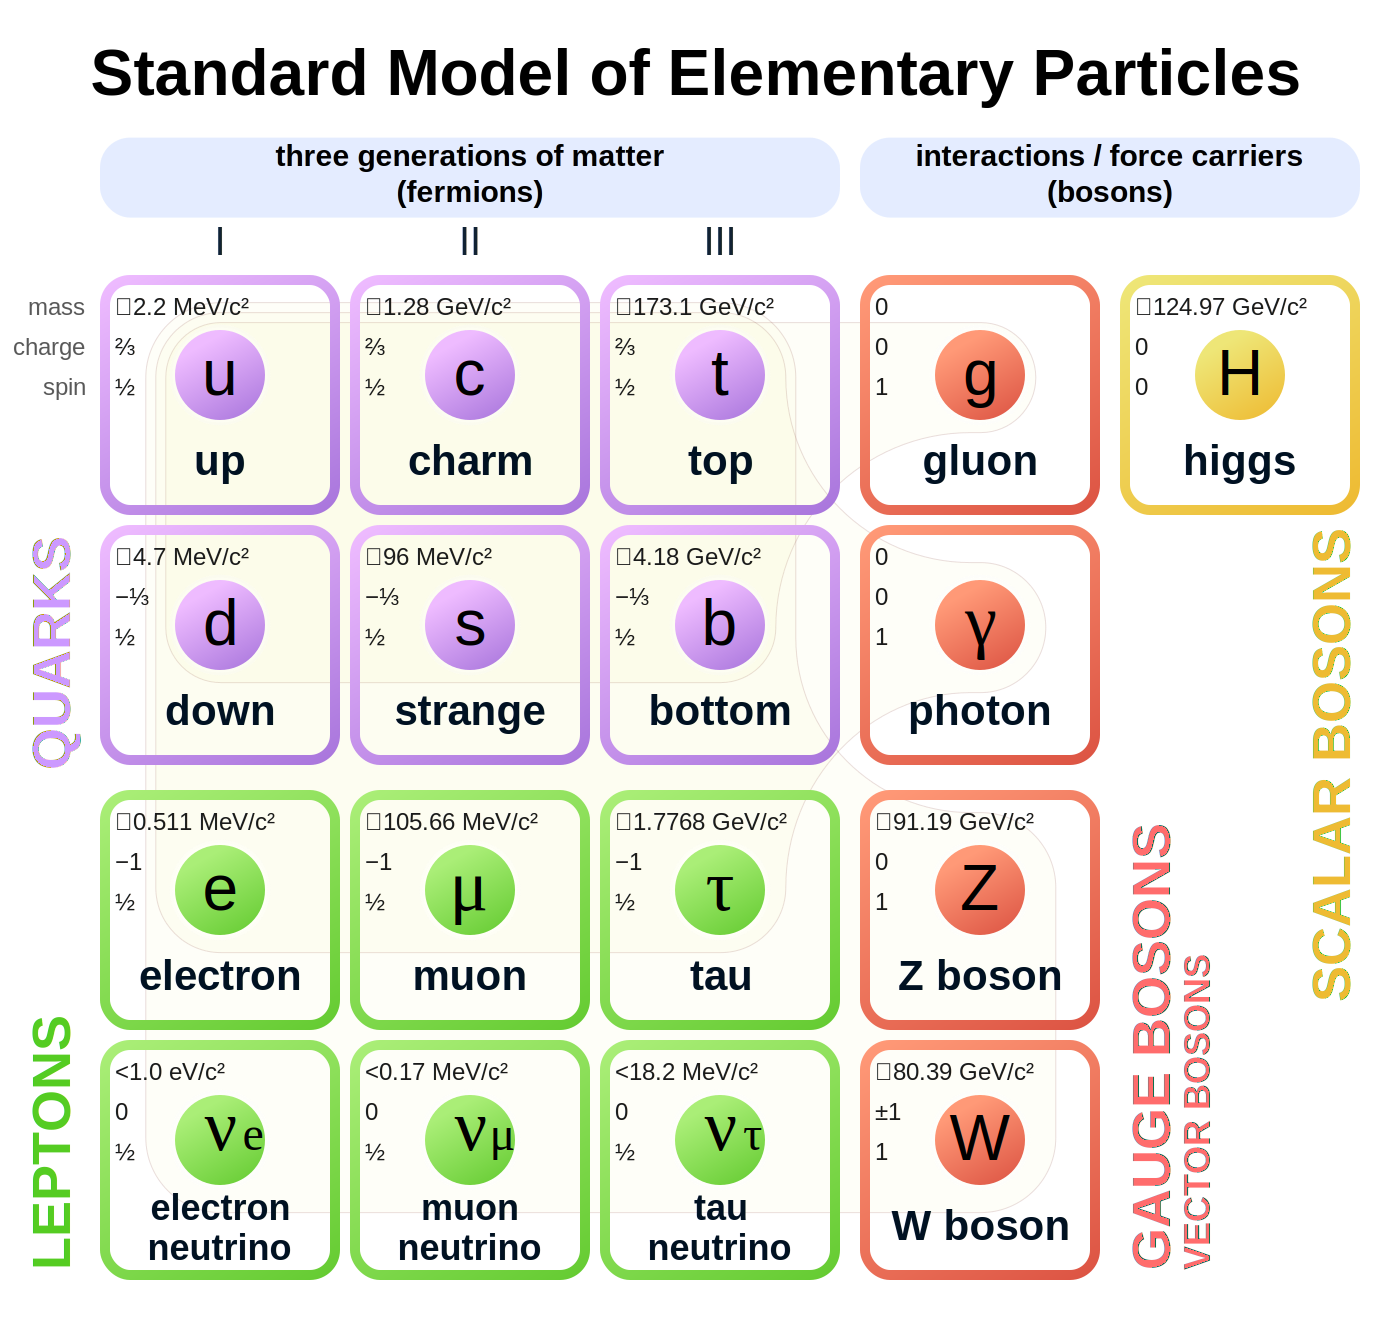
\includegraphics[scale=0.25]{Figures/StandardModel}
\decoRule
\caption{Standard model of particle physics \cite{SMwiki}.}
\label{fig:StandardModel}
\end{figure}

\subsection{Fermions (Quarks and Leptons)}
There are six quarks (up \textit{u}, down \textit{d}, charm \textit{c}, strange \textit{s}, top \textit{t}, bottom \textit{b}) and six leptons (electron $e^{-}$, electron neutrino $\nu_{e}$, muon $\mu^{-}$, muon neutrino $\nu_{\mu}$, tau $\tau^{-}$, tau neutrino $\nu_{\tau}$) divided into pairs of particles in three generations, see figure \ref{fig:StandardModel}. Each particle carries more mass than the corresponding previous generation particle. The first generation particles do not decay, and they form all the visible matter. The quarks carry a color charge (red, blue, green), and anti-quarks carry an anti-color charge (anti-red, anti-blue, anti-green). The color charge in quarks allows them to interact via strong force that only affects the particle with color charge. Due to the color confinement, there is a tight bond between quarks with the strong force. The quarks always form a color-neutral bound state, baryon (\textit{qqq} or $\overline{q}\overline{q}\overline{q}$), or meson ($q\overline{q}$). The color neutral means either a color and anti-color (e.g, blue and anti-blue) or sum of the three colors or anti-colors (e.g, red and blue and green). Which means, proton (\textit{p}) is a composite of three quarks with different color charges ($u_{r}u_{g}d_{b}$ and all the other possible colorless combinations). All fermions have the corresponding anti-fermion with the opposite charge to the fermion.

\subsection{Bosons}

The intermediate vector bosons (gauge bosons) are the force carriers for the SM interactions (strong, weak, electromagnetic). The SM gauge bosons are as follows:  

\begin{itemize}
\item \textbf{Photon ($\gamma$)}: It mediates the electromagnetic interactions between the electrically charged particles, the interactions described by QED (Quantum Electrodynamics). The photon rest mass is zero and has no electric or color charge.

\item \textbf{$W^{\pm}$ and $Z^{0}$ bosons}: These bosons are the mediators of the weak force between all fermions. The $W^{\pm}$ ($\sim80GeV$) and $Z^{0}$ ($\sim90GeV$) are very massive. As W has +1 or -1 electric charge, it participates in the electromagnetic interaction. The electroweak theory describes combined weak and QED interactions.

\item \textbf{Gluons}: There is a total of eight gluons. They are massless carriers of the strong interaction between quarks and gluons. They carry a pair of color-anti-color charges (e.g., blue-antired) but have no electric charge. The gluons have self-interaction because they have a color charge. The theory describes strong interactions is QCD (Quantum Chromodynamics).

\end{itemize}

There is only one scalar boson (spin = 0) predicted by the SM, the Higgs boson ($H$). The Higgs mechanism is essential to explain the mass of the gauge bosons. In QFT, without the Higgs mechanism, all intermediate bosons considered massless.  So the massive $W^{\pm}$ and $Z^{0}$ bosons could not be explained without having a Higgs mechanism that gives mass to the $W^{\pm}$ and $Z^{0}$ bosons. 

\subsection{Interactions}

\begin{figure}
\centering
\feynmandiagram [vertical = b to a] {
	i1 [particle=\(e^{-}\)]
	-- [anti fermion] a
	-- [anti fermion] f1 [particle=\(e^{-}\)],
	a -- [photon, edge label=\(\gamma\)] b,
	i2 [particle=\(e^{-}\)]
	-- [fermion] b
	-- [fermion] f2 [particle=\(e^{-}\)],
};
\decoRule
\caption{Feynman diagram of electron-electron scattering. The diagram shows the two incoming $e^{-}$ from left, exchange a photon and scatter of to right.}
\label{fig:Feynman_ee}
\end{figure}

In the SM, each interaction is described by the corresponding Quantum Field Theory (QFT). The interaction takes place by exchanging one of the spin-1 gauge bosons. In QED, the interaction between charged particles mediated by the exchange of photons ($\gamma$). As an example, in the electron-electron scattering process, a photon ($\gamma$) is emitted by one of the incoming electrons ($e$) and absorbed by the other one, see figure \ref{fig:Feynman_ee}. The weak charged interactions mediated by the charged $W^{+}$ and $W^{-}$ bosons, the nuclear beta decay is an example of weak charged interaction. The weak neutral interactions take place by exchanging Z bosons. The strong interaction described by QCD mediated by exchanging the gluons (e.g., quark-quark scattering process). 

The electromagnetic force is the force that acts between electrically charged particles. It has an infinite range, unlike weak and strong are very short-range interactions (sub-atomic). The signature of the weak interactions is CP-symmetry (charge conjugation parity symmetry) violation, but CPT-symmetry (charge, parity, and time reversal symmetry) is conserved in the weak interaction. All fermions carry a property called iso-spin which allows them to interact via the weak force. The strong interaction is a very short-range force that acts only on the particles that carry the color charge. The quarks and gluons can interact with the strong force.

\begin{table}[H]
\caption{Fundamental interactions strength comparison \cite{Interactions}.}
\label{tab:FundamentalInteractions}
\centering
\begin{tabular}{l l l}
\toprule
Force & Strength & Mediator \\
\midrule
Strong & \(10\) & Gluon\\
Electromagnetic & \(10^{-2}\) & Photon\\
Weak & \(10^{-13}\) & W and Z \\
Gravity & \(10^{-42}\) & Graviton\\
\bottomrule\\
\end{tabular}
\end{table}

\section{The Top Quark}
\label{TopQ}

The detection of heavy hadrons confirmed the existence of heavy quarks. The top quark was not discovered until 1995, and all the early searches failed to detect the top baryon or meson. Unlike the other five quarks, the top quark is so heavy ($\sim174GeV$) and has a very short lifetime, it does not form any bound state of mesons or baryons. In other words, the top quark does not hadronize, so it not possible to see any top-hadron. This implies that the top quark decays before it gets confined by passing its spin information to its decay products. Additionally, this also enables the possibility of studying the polarization of the \textit{W}-boson from the top quark.

The detection of the top quark, in 1995 through the CDF \cite{PhysRevLett.74.2626} and DØ \cite{PhysRevLett.74.2632} experiments on the TEVATRON accelerator at the FERMILAB, turned into a significant achievement on the way of completing the missing portions of a beautiful puzzle, the SM. The reaction to produce top quark was $u+\overline{u} \rightarrow t+\overline{t}$ ; The analysis of decay products lead to the discovery as the \textit{t} and $\overline{t}$ are very short-lived to be detected. The top quark was theoretically hypothesized with the bottom quark (\textit{b}), in 1973 by Kobayashi and Maskawa \cite{10.1143/PTP.49.652}, and they complete the third generation of quark family. 
%The top quark is the most massive (strong coupling to the Higgs) SM particle, and it is probably unique among all quarks and leptons and might play a role within the mechanism of electroweak symmetry breaking.

\subsection{Top Quark Production and Decay}
\label{TopQproductiondecay}

Top quarks at LHC can be produced as single top quarks via weak interaction or as top anti-top quark pairs production via strong interaction. The top quark pair production is the dominant process at the LHC. Top quark pairs can be produce via two different processes: gluon-gluon fusion and quark-antiquark annihilation. The quark-antiquark annihilation is suppressed by gluon-gluon fusion (approximately $90\%$) at LHC because the anti-quark only comes from the sea-quarks of proton. The leading order feynman diagrams of top quark pair production are given in \ref{fig:toppairproduction}.
 
\begin{figure}[H]
\centering
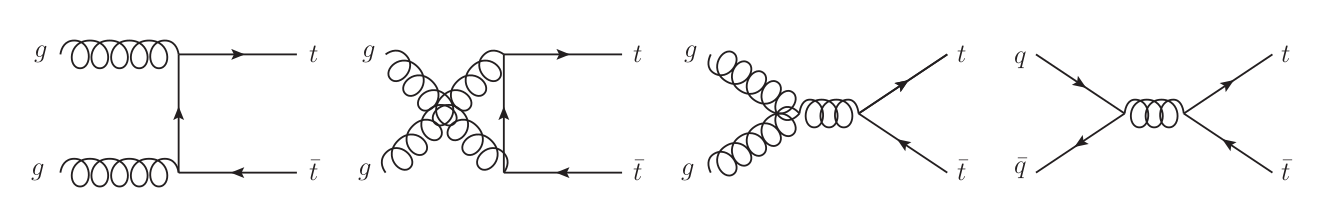
\includegraphics[scale=0.3]{Figures/top_pair_production.png}
\decoRule
\caption{Representative Feynman diagrams for top anti-top quark pair production at the leading order QCD matrix element. From the left, the first three correspond to the gluon-gluon fusion and the last one represents the quark anti-quark annihilation\cite{borathesis1}.}
\label{fig:toppairproduction}
\end{figure} 

Single top quark production is an electroweak interaction and mostly associated with \textit{b} quark and \textit{W}\textit{} boson (Wtb vertex). The process is dominated by t-channel (almost $70\%$) at $\sqrt{s}=13$TeV at the LHC. The feynman diagrams for the t-channel and s-channel process are given in \ref{fig:singletopproduction}.

\begin{figure}[H]
\centering
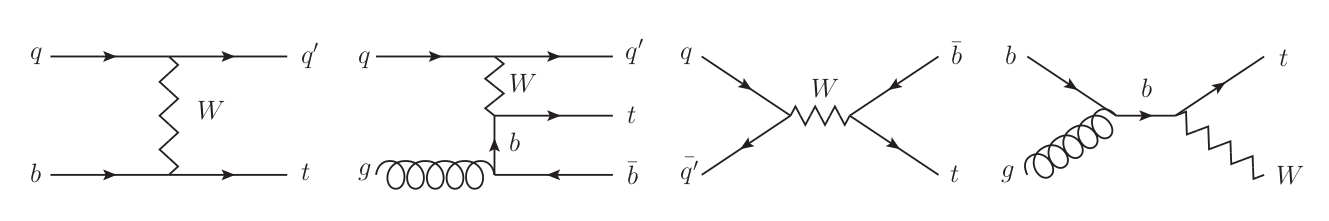
\includegraphics[scale=0.3]{Figures/single_top.png}
\decoRule
\caption{Feynman diagrams for single top quark production at leading order matrix element. From the left, the first two diagram represent the t-channel production. The third diagram is the s-channel production and the last one is the W t-channel production\cite{borathesis1}.}
\label{fig:singletopproduction}
\end{figure}

The top quark lifetime is shorter than the hadronization time and it decays almost $100\%$ into a bottom quark and a \textit{W}-boson. Therefore, the decay modes are classified depending on further decays of daughter \textit{W}'s into: hadronic channel, dileptonic channel and semileptonic channel.

\begin{figure}[H]
\centering
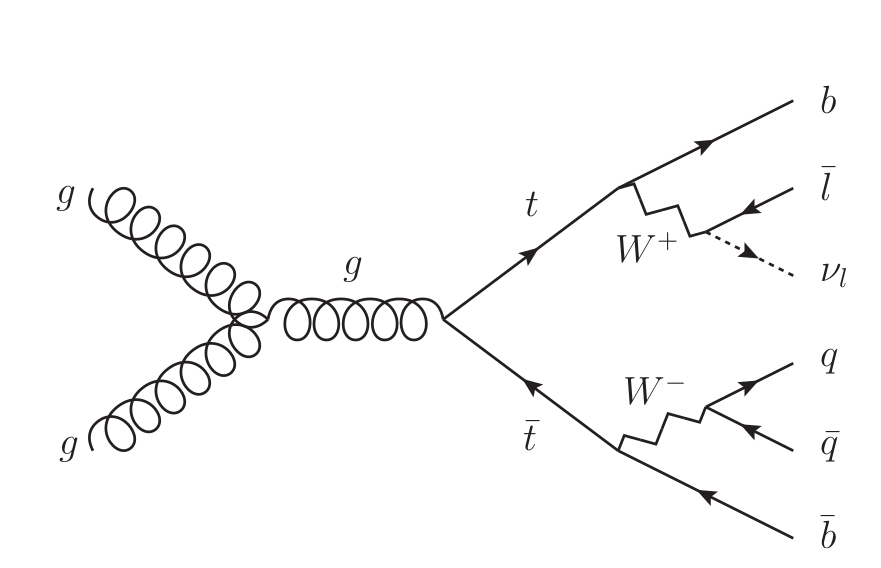
\includegraphics[scale=0.3]{Figures/top_decay.png}
\decoRule
\caption{Feynman diagrams for semileptonic decay channel of top-anti-top quarks\cite{borathesis1}.}
\label{fig:topdecay}
\end{figure}

\textbf{Hadronic decay channel}: Both \textit{W}-bosons decay into quark-anti-quark pairs and the final state has a total of six jets in which two of them are b-jets. The branching ratio of this channel is around $46\%$ but the final state has large background due to six final state jets.

\textbf{Dileptonic decay channel}: Both \textit{W}-boson decay into a lepton and lepton neutrino. The final state is very clean as compare to fully hadronic decay but the branching ratio is around $10\%$ which is very small. Also the two neutrinos in the final state can make the analysis more difficult (neutrino cannot be detected by ATLAS and only can be identified by missing energy at the final state).

\textbf{Semileptonic decay channel}: One of the \textit{W}-boson's decay hadronically and the other one leptonically. The branching ratio of the decay channel is around $43\%$ and the final state is cleaner (4-jets) as compare to fully hadronic decay. The Feynman diagram of the process represented in Figure \ref{fig:topdecay}.

\begin{figure}[H]
\centering
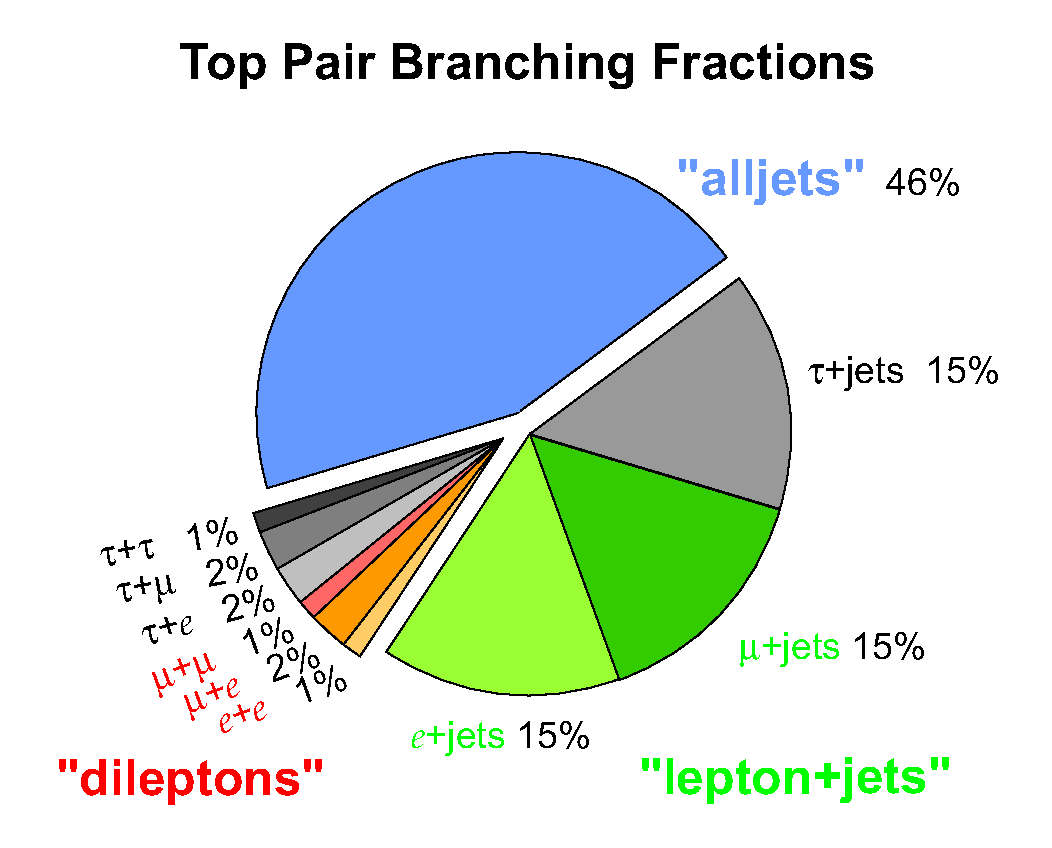
\includegraphics[width=10cm]{Figures/top_pair_branching_frac.eps}
\decoRule
\caption{Top-anti-top quark pair decay channels and the pie chart with branching fractions. The decay channels are categorized depending on the the further decay of $W^{\pm}$ into quarks or leptons\cite{toppair-branching}.}
\label{fig:topdecaychannels}
\end{figure}

\subsection{Top Quark Associated with Photon}
\label{ttgamma}

Measurements of the top quark's coupling to vector bosons have great importance to test the SM and any deviation from SM can give a hint about beyond standard model underlying theories. The top quark coupling with photon is our interest which theoretically, can be measured from the top quark pair production via photon. The $q\overline{q} \rightarrow \gamma \rightarrow t\overline{t}$ cannot be observed directly at LHC because the top quark pair production is dominated by gg-fusion ($\sim90\%$). The remaining $\sim10\%$ for $q\overline{q}$ annihilation can be mediated by $g$, $Z$ and $\gamma$; And the production mediated by gluon is the dominating process so the \textit{t} coupling with $\gamma$ cannot be probed directly. There are two other processes, top quark pair production with photon: the radiative top quark production and the radiative top decay. top quark pair production in association with a photon is our interest and in the following briefly the radiative $t\overline{t}$ production and decay has been discussed. Photon can be radiated of top quark in the pair production or in the decay process of the the top quark.

In the radiative $t\overline{t}$ production process via $q\overline{q}$ annihilation, the photon can decay from one of the incoming or outgoing quarks. In the gluon gluon fusion process, the photon only can be radiated of one of the top quarks. The respective Feynman diagrams are shown in figure \ref{fig:feynmanttgamma1} for illustration.

\begin{figure}[H]
\centering
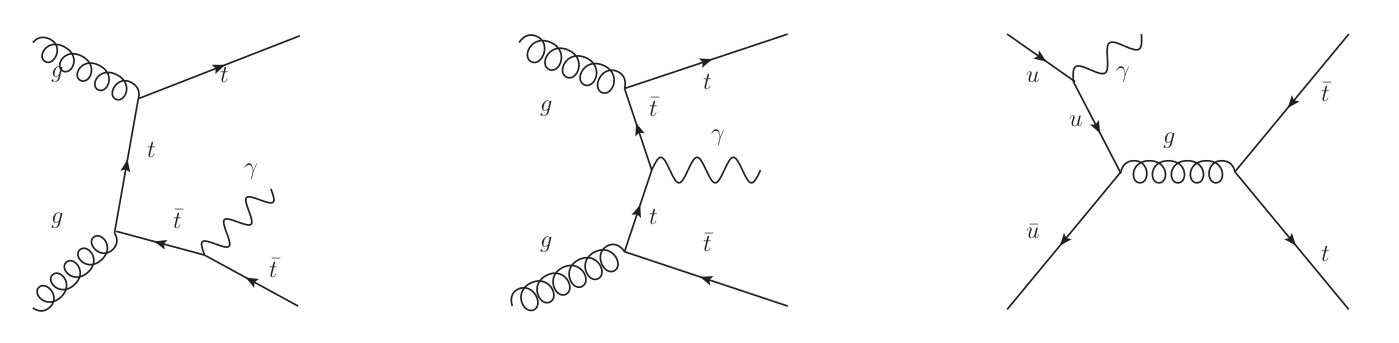
\includegraphics[width=14cm]{Figures/ttgamma_production.png}
\decoRule
\caption{Representative Feynman diagrams for radiative top quark pair production \cite{borathesis1}.}
\label{fig:feynmanttgamma1}
\end{figure}

The photon in the radiative $t\overline{t}$ decay, can be radiated from the top quark or one of the top quark decay products: bottom-quark, \textit{W}-boson and the leptons from \textit{W}-decay. The respective Feynman diagrams are given in the figure \ref{fig:feynmanttgamma2}. The top-photon coupling is our topic of interest but experimentally we cannot distinguish the photons from radiative production or decay.

\begin{figure}[H]
\centering
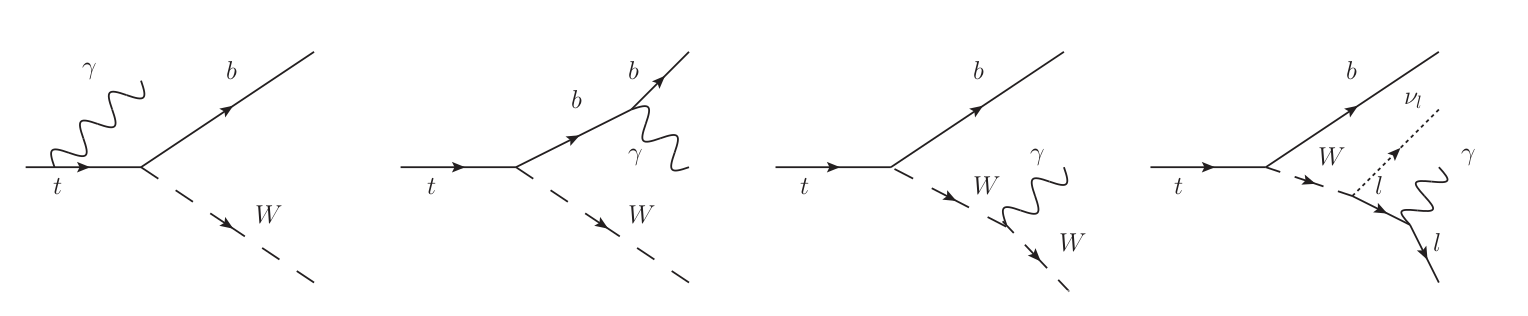
\includegraphics[width=14cm]{Figures/ttgamma_decay.png}
\decoRule
\caption{Representative Feynman diagrams for radiative top quark decay\cite{borathesis1}.}
\label{fig:feynmanttgamma2}
\end{figure}